\documentclass{article}
\usepackage[LGR, T1]{fontenc}
\usepackage[greek]{babel}
\usepackage{cancel}
\usepackage{amsmath}
\usepackage{tikz}
\usepackage{alltt}
\usetikzlibrary{shapes.geometric}
\usetikzlibrary{trees}
\begin{document}
\title{\textlatin{question4}}
\maketitle

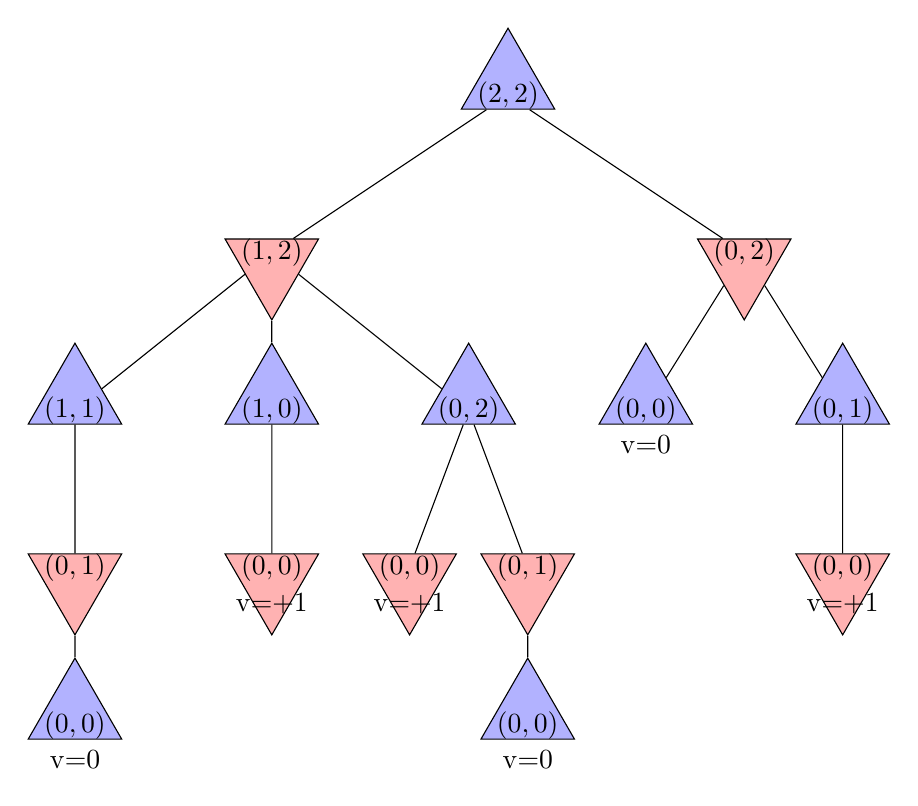
\begin{tikzpicture}[
  max/.style={draw, fill=blue!30, isosceles triangle, isosceles triangle apex angle=60, shape border rotate=90, minimum size=1cm, inner sep=0pt},
  min/.style={draw, fill=red!30, isosceles triangle, isosceles triangle apex angle=60, shape border rotate=270, minimum size=1cm, inner sep=0pt},
  level 1/.style={sibling distance=60mm},
  level 2/.style={sibling distance=25mm},
  level 3/.style={sibling distance=15mm},
  level distance=20mm
]

% Root node (Max node)
\node[max] {$(2, 2)$}
  % Level 1
  child {node[min] {$(1, 2)$}
    % Level 2
    child {node[max] {$(1, 1)$}
      % Level 3
      child {node[min] {$(0, 1)$}
        child {node[max] {$(0, 0)$} node[below=2mm] {\textlatin{v}=0}}
      }
    }
    child {node[max] {$(1, 0)$}
      child {node[min] {$(0, 0)$} node[below=2mm] {\textlatin{v}=+1}}
    }
    child {node[max] {$(0, 2)$}
      child {node[min] {$(0, 0)$}node[below=2mm] {\textlatin{v}=+1}}
      child {node[min] {$(0, 1)$} 
      child {node[max] {$(0, 0)$} node[below=2mm] {\textlatin{v}=0}}
      }
    }
  }
  child {node[min] {$(0, 2)$}
    % Level 2
    child {node[max] {$(0, 0)$} node[below=2mm] {\textlatin{v}=0}}
    child {node[max] {$(0, 1)$}
      child {node[min] {$(0, 0)$} node[below=2mm] {\textlatin{v}=+1}}
    }
  };
\end{tikzpicture}
\pagebreak

Παραπάνω φαίνεται το δέντρο παιχνιδιού για την έκδοση του \textlatin{Nim game} όπως περιγράφεται στην εκφώνηση.\\
\\
Έπειτα, θα αριθμίσουμε τους κόμβους ώστε να τρέξουμε θεωρητικά τον αλγόριθμο \textlatin{alpha-beta pruning} (κλάδεμα άλφα-βητα), παρόμοια όπως στην δεύτερη άσκηση. Όμοια, η στοίχιση των γραμμών είναι πολύ σημαντική καθώς δηλώνει το βάθος και σε ποιο α-β αναφερόμαστε.

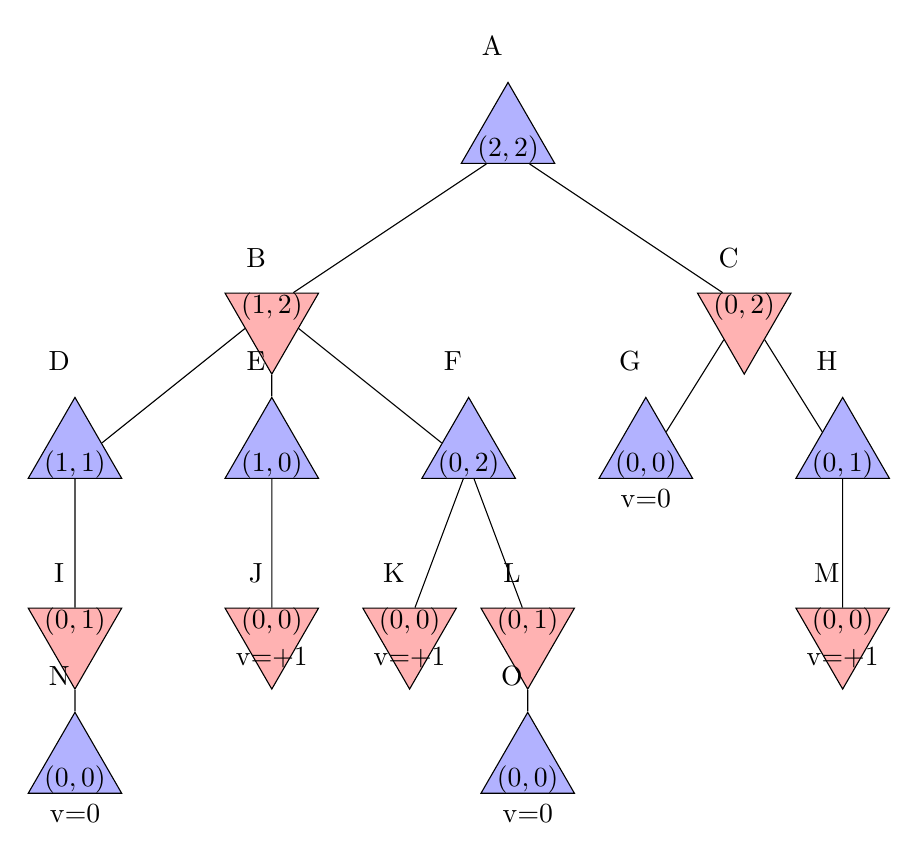
\begin{tikzpicture}[
  max/.style={draw, fill=blue!30, isosceles triangle, isosceles triangle apex angle=60, shape border rotate=90, minimum size=1cm, inner sep=0pt},
  min/.style={draw, fill=red!30, isosceles triangle, isosceles triangle apex angle=60, shape border rotate=270, minimum size=1cm, inner sep=0pt},
  level 1/.style={sibling distance=60mm},
  level 2/.style={sibling distance=25mm},
  level 3/.style={sibling distance=15mm},
  level distance=20mm
]

% Root node (Max node)
\node[max, label={[shift={(-0.2,0.2)}]above:\textlatin{A}}] {$(2, 2)$}
  % Level 1
  child {node[min, label={[shift={(-0.2,0.2)}]above:\textlatin{B}}] {$(1, 2)$}
    % Level 2
    child {node[max, label={[shift={(-0.2,0.2)}]above:\textlatin{D}}] {$(1, 1)$}
      % Level 3
      child {node[min, label={[shift={(-0.2,0.2)}]above:\textlatin{I}}] {$(0, 1)$}
        child {node[max, label={[shift={(-0.2,0.2)}]above:\textlatin{N}}] {$(0, 0)$} node[below=2mm] {\textlatin{v}=0}}
      }
    }
    child {node[max, label={[shift={(-0.2,0.2)}]above:\textlatin{E}}] {$(1, 0)$}
      child {node[min, label={[shift={(-0.2,0.2)}]above:\textlatin{J}}] {$(0, 0)$} node[below=2mm] {\textlatin{v}=+1}}
    }
    child {node[max, label={[shift={(-0.2,0.2)}]above:\textlatin{F}}] {$(0, 2)$}
      child {node[min, label={[shift={(-0.2,0.2)}]above:\textlatin{K}}] {$(0, 0)$}node[below=2mm] {\textlatin{v}=+1}}
      child {node[min, label={[shift={(-0.2,0.2)}]above:\textlatin{L}}] {$(0, 1)$} 
      child {node[max, label={[shift={(-0.2,0.2)}]above:\textlatin{O}}] {$(0, 0)$} node[below=2mm] {\textlatin{v}=0}}
      }
    }
  }
  child {node[min, label={[shift={(-0.2,0.2)}]above:\textlatin{C}}] {$(0, 2)$}
    % Level 2
    child {node[max, label={[shift={(-0.2,0.2)}]above:\textlatin{G}}] {$(0, 0)$} node[below=2mm] {\textlatin{v}=0}}
    child {node[max, label={[shift={(-0.2,0.2)}]above:\textlatin{H}}] {$(0, 1)$}
      child {node[min, label={[shift={(-0.2,0.2)}]above:\textlatin{M}}] {$(0, 0)$} node[below=2mm] {\textlatin{v}=+1}}
    }
  };
\end{tikzpicture}

\newpage

\begin{alltt}
Επισκεπτόμαστε τον κόμβο \textlatin{A} (\textlatin{MAX}) [α=-\(\infty\), β=\(\infty\)]
  Επισκεπτόμαστε τον κόμβο \textlatin{B} (\textlatin{MIN}) [α=-\(\infty\), β=\(\infty\)]
    Επισκεπτόμαστε τον κόμβο \textlatin{D} (\textlatin{MAX}) [α=-\(\infty\), β=\(\infty\)]
      Επισκεπτόμαστε τον κόμβο \textlatin{I} (\textlatin{MIN}) [α=-\(\infty\), β=\(\infty\)]
        Επισκεπτόμαστε το φύλλο \textlatin{N} (\textlatin{MAX}) με τιμή 0
      \textlatin{Updated} α=-\(\infty\), β=0
      Ο κόμβος \textlatin{I} παίρνει την τιμή: 0
    \textlatin{Updated} α=0, β=\(\infty\)
    Ο κόμβος \textlatin{D} παίρνει την τιμή: 0
  \textlatin{Updated} α=-\(\infty\), β=0
    Επισκεπτόμαστε τον κόμβο \textlatin{E} (\textlatin{MAX}) [α=-\(\infty\), β=0]
      Επισκεπτόμαστε το φύλλο \textlatin{J} (\textlatin{MIN}) με τιμή 1
    \textlatin{Updated} α=1, β=0
    Ο κόμβος \textlatin{E} παίρνει την τιμή: 1
    Επισκεπτόμαστε τον κόμβο \textlatin{F} (\textlatin{MAX}) [α=-\(\infty\), β=0]
      Επισκεπτόμαστε το φύλλο \textlatin{L} (\textlatin{MIN}) με τιμή 1
    \textlatin{Updated} α=1, β=0
    Κλαδέυονται 1 υπολοιπόμενο/α παιδία του \textlatin{F} - Beta cutoff, το/τα οποίο/α είναι: \textlatin{K}
    Ο κόμβος \textlatin{F} παίρνει την τιμή: 1
  Ο κόμβος \textlatin{B} παίρνει την τιμή: 0
\textlatin{Updated} α=0, β=\(\infty\)
  Επισκεπτόμαστε τον κόμβο \textlatin{C} (\textlatin{MIN}) [α=0, β=\(\infty\)]
    Επισκεπτόμαστε τον κόμβο \textlatin{H} (\textlatin{MAX}) [α=0, β=\(\infty\)]
      Επισκεπτόμαστε το φύλλο \textlatin{M} (\textlatin{MIN}) με τιμή 1
    \textlatin{Updated} α=1, β=\(\infty\)
    Ο κόμβος \textlatin{H} παίρνει την τιμή: 1
  \textlatin{Updated} α=0, β=1
    Επισκεπτόμαστε το φύλλο \textlatin{G} (\textlatin{MAX}) με τιμή 0
  \textlatin{Updated} α=0, β=0
  Ο κόμβος \textlatin{C} παίρνει την τιμή: 0
Ο κόμβος \textlatin{A} παίρνει την τιμή: 0
\end{alltt}

Η τιμή \textlatin{minimax} στη ρίζα του δέντρου παιχνιδιού είναι 0, που σημαίνει ότι αν και οι δύο παίκτες παίζουν βέλτιστα, το αποτέλεσμα είναι νίκη για τον \textlatin{MIN} από άποψη χρησιμότητας (έχουμε ορίσει 0 για τις καταστάσεις που κερδίζει ο \textlatin{MIN}, αντίστοιχα 1 για \textlatin{MAX}).
Μια τιμή \textlatin{minimax} 0 με άλλα λόγια υποδηλώνει ότι ο \textlatin{MIN} θα κερδίσει, καθώς ο \textlatin{MAX} δεν μπορεί να επιβάλει χρησιμότητα +1 ακόμα και αν παίξει βέλτιστα (εφ'όσον και ο \textlatin{MIN} παίξει βέλτιστα).
\end{document}
